
\chapter{Sicherheit} 

Im folgenden Kapitel wird ein Konzept von Sicherheitsmechanismen vorgestellt,
welches f\"ur eine sichere Daten\"ubertragung zwischen der Anwendersoftware und Web- bzw. Datenbankserver sorgen soll.
Eine Webanwendung ist eine Software, die beim Benutzer im Webbrowser abl\"auft. 
Sie kommuniziert dabei \"uber das Internet mit einem Server, von dem aus sie gestartet wird.
Einige Anwendungen auf einem lokalen Rechner oder Smartphone erfordern f\"ur ihre Funktionalit\"at ebenfalls eine Verbindung zum Internet
und tauschen in vielen F\"allen sensible Informationen aus.
Diese Daten m\"ussen vor unbefugtem Zugriff und Einsicht durch Dritte gesch\"utzt werden.
Zum Schutz der Daten\"ubertragung werden verschiedene Schutzmechanismen eingesetzt. 
\cite[S. 499]{PHP_MySQL:01} \cite{Sicherheit:01}\\

\section{Verschl\"usselung}

Unter \emph{Verschl\"usselung} versteht man eine Klartextnachricht mittels Kryptographie in eine unleserliche Form zu bringen.
F\"ur diesen Vorgang gibt es Ein-Weg- und Zwei-Wege-Verschl\"usselungen.
Die Ein-Weg-Verschl\"usselung chiffriert eine Nachricht nur in eine Richtung. 
Das bedeutet, diese kann nicht mehr entschl\"usselt werden.
Diese Eigenschaft wird genutzt, um zum Beispiel Passw\"orter nicht als Klartext,
sondern als eine Pr\"ufsumme \"uber das Netzwerk zu \"ubertragen.
Auf diese Weise ist es f\"ur einen Angreifer beim Abfangen der \"Ubertragung im Internet oder direkten Zugriff
auf die Datenbank nicht m\"oglich das Passwort in Klartext zu lesen.
Diese Art der Verschl\"usselung wird auch als Hashing-Verfahren bezeichnet.
Bei dem Verfahren der Zwei-Wege-Verschl\"usselung wird eine Nachricht verschl\"usselt und beim Empf\"anger wieder entschl\"usselt.\\

\subsection{MD5}
Ein aktuelles Hashing-Verfahren ist MD5. 
Das steht f\"ur \emph{Message Digest Version 5}\cite[S. 507]{PHP_MySQL:01}.
Beim Verschl\"usseln erzeugt MD5 aus einer Zeichenkette von beliebiger L\"ange einen 128-Bit-Hashwert und stellt diesen hexadezimal dar.
In der Abbildung 3.1 wird ein m\"oglicher Hashwert aus dem String \dq Dawid Janas\dq{} dargestellt.\\

\begin{figure}[h]
  \centering
  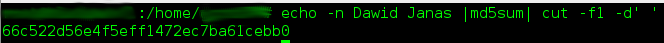
\includegraphics[scale=0.6]{fotos/kapitel3/md5sum.png}
  \caption{MD5 Hash aus dem String \dq Dawid Janas\dq{}}
 
\end{figure}

\subsection{SHA}
Ein weiteres Ein-Weg-Verschl\"usselungsverfahren ist SHA. 
SHA ist eine Alternative zu MD5 und steht f\"ur \emph{Secure Hash Algorithm}.
In der Regel wird aus der SHA-Familie das SHA1 Verfahren genutzt. 
Neben diesen existieren noch weitere Algorithmen wie SHA256 oder SHA512 und sollen in der Zukunft SHA1
als Standard ersetzen.
SHA1 erzeugt einen 40-Bit langen Hashwert und ist im Gegensatz zu MD5 robuster gegen Brute-Force-Attacken.
Aktuell sind MD5 und SHA1 zum Schutz ausreichend.
Der Zeitaufwand, um deren Verschl\"usselung zu brechen, ist heute noch zu gro\ss{}, so dass sie mit ruhigem Gewissen genutzt werden k\"onnen.\\

\subsection{Zwei-Wege-Verschl\"usselung}

Bei der Entwicklung von Anwendungen, bei denen es notwendig ist kryptographische Mechanismen zu benutzen, gibt es zahlreiche Optionen.
Die Entwicklungswerkzeuge f\"ur Android bieten von Haus aus Pakete wie \emph{javax.crypto} oder \emph{java.security},
welche Schnittstellen und Klassen mit Algorithmen f\"ur Verschl\"usselung oder Zertifikat- und Signaturverifizierung bereitstellen, an.\\

Die Sprache PHP stellt f\"ur die Verschl\"usselung das Modul \emph{mcrypt} bereit\cite[S. 510]{PHP_MySQL:01}.\\
Dieses Modul stellt unter anderem folgende Verschl\"usselungsalgorithmen zur Verf\"ugung:
\begin{itemize}
 \item Blowfish: ist ein Blockverschl\"usselungsalgorithmus mit einer Schl\"ussell\"ange zwischen 32-Bit und 448-Bit.
 \item (Triple-)DES: symmetrischer Verschl\"usselungsalgorithmus mit einer Schl\"ussell\"ange von 168-Bit.
 \item Rijndael-Algorithmen: auch genannt Advanced Encryption Standard (AES). 
 Die Variante AES-192 und AES-256 sind in den USA f\"ur die Verschl\"usselung von staatlichen Dokumenten zugelassen\cite{Sicherheit:05}.
 
\end{itemize}




\section{TLS/SSL}
Zum Versenden von Daten \"uber das Internet bietet das HTTP-Protokoll die zwei Methoden GET und POST zur Auswahl.
Beide senden Daten im Klartext. F\"ur neugierige Augen scheint die Methode POST sicherer zu sein als GET.
Das liegt daran, dass GET die Formulardaten einfach an die URL in der Adressleiste anh\"angt.
Bei POST sind die Daten nicht sichtbar, da sie im HTTP-Header versteckt werden.
Mittels \emph{Sniffing} lassen sich HTTP-Header leicht abfangen und Werkzeuge, wie Wireshark, machen den gesamten Datenverkehr
f\"ur den Angreifer sichtbar.
Um ungewolltes Mitlesen zu verhindern, ist es notwendig den Datenverkehr \"uber eine sichere Leitung und verschl\"usselt zu schicken.
F\"ur diesen Zweck setzt man f\"ur die Kommunikation SSL/TLS ein.
SSL steht f\"ur \emph{Secure Socket Layer} \cite[S. 513]{PHP_MySQL:01}\cite[S. 766]{Sicherheit:04} und TLS f\"ur \emph{Transport Layer Security}\cite{Sicherheit:03}.
Dabei ist TLS eine modifizierte Version von SSL Version 3.
Beide Protokolle werden heute von allen Browsern und Servern unterst\"utzt.
Sie sorgen f\"ur Vertraulichkeit, Datenintegrit\"at und Endpunktauthentifizierung, w\"ahrend einer Verbindung zwischen Client und Server.
T\"atigt man heute einen Einkauf im Internet und bezahlt mit Kreditkarte, so wird mit Sicherheit SSL eingesetzt.
Man erkennt dies daran, dass die URL der Webseite nicht mit \emph{http}, sondern mit \emph{https} beginnt.
SSL kann von jeder Anwendung genutzt werden, die \"uber TCP kommuniziert.
\"Uber entsprechende Bibliotheken hat man Zugriff auf die SSL-Socket-Schnittstelle.
Die Programmierung ist analog zur TCP-Anwendungsprogrammierschnittstelle (TCP-API).
TLS/SSL nutzt ein hybrides Verschl\"usselungsverfahren aus Ein- und Zwei-Wege-Verschl\"usselungen.
Beim Aufbau einer Verbindung stellt der Client eine TCP-Verbindung zum Server auf.
Als n\"achstes \"uberpr\"uft der Client, ob der Server wirklich der ist, als wen er sich ausgibt.
Dies geschieht mittels eines Zertifikats, welches den Eigent\"umer best\"atigt.
Ein solches Zertifikat bekommt man gegen Geld bei entsprechenden Zertifizierungsstellen.
Dabei sollte nicht vergessen werden,dass selbsterstellte, nicht beglaubigte Zertifikate von der Android-Plattform verweigert werden\cite[S. 356]{Android:02}.
Beim Verbindungsaufbau sendet der Server sein Zertifikat an den Client.
Gleichzeitig bekommt der Client auch einen \"offentlichen Schl\"ussel vom Server, mit dem er den Rest der Kommunikation verschl\"usselt.
Der Client generiert nun ein so genanntes \emph{Master Secret} und sendet es an den Server.
Mit dem Master Secret berechnen nun Server und Client verschiedene Schl\"ussel f\"ur Chiffren und die Integrit\"atspr\"ufung.
W\"ahrend der Kommunikation werden die Datenpakete mit Sequenznummern versehen, um sie vor Manipulation von Au\ss{}en zu sch\"utzen.\\



\section{Sicherheitskonzept}

Ein wichtiger Punkt in der Bachelorarbeit ist das Sicherheitskonzept.
Der Patient protokolliert Informationen \"uber sein Essverhalten und seinen Gesundheitszustand.
Sein Arzt unterliegt der \"arztlichen Schweigepflicht.
Demselben Grundsatz unterliegt die Software.
Somit m\"ussen die Tagesprotokolle des Patienten beim \"Ubertragen und Persistieren vor Einsicht durch Dritte gesch\"utzt werden.
Die gesamte Anwendung, sprich Android-Anwendung, Web-Anwendung, Anwendungsserver und Datenbankserver bilden eine 3-Tier-Architektur.
Hier findet ein Datenfluss \"uber unsichere Medien, wie das Internet und ein Intranet, statt.
Um f\"ur eine sichere Behandlung der Daten zu sorgen, m\"ussen aus diesem Grund an mehreren Stellen der Software unterschiedliche Sicherheitsmechanismen angewandt werden.\\

\subsection{Web-API}

Der Zugriff auf die Funktionalit\"at der Webanwendung erfolgt \"uber eine Zugriffs-API.
Der Client ruft nicht direkt eine PHP-URL mit einem Skript, welches die gew\"unschte Funktion erf\"ullt, auf,
sondern \"ubergibt einen Schl\"ussel als Parameter und sendet die Anfrage \"uber GET oder POST an die Zugriffs-API.
Dieser Schl\"ussel ist an die gew\"unschte Funktion auf der Serverseite gebunden.
Zum Beispiel will der Client Informationen \"uber alle Patientennamen erhalten.
F\"ur diesen Fall ist die Anfrage im Listing 3.1 demonstriert.\\

\begin{lstlisting}[caption={Beispiel f\"ur einen Zugriff \"uber eine Zugriffs-API}]
// pseudo code
parameter = "get_all_patientennamen" + "myUserName" + "myPassword" + "api_key";
patientenNamen = HTTP.post("web_api.php", "parameter");
\end{lstlisting}

Die Zugriffs-API \"uberpr\"uft die Parameter.
Der Parameter \emph{api\_key} muss ein g\"ultiger Schl\"ussel f\"ur die Web-API sein.
Dieser Schl\"ussel best\"atigt, dass der Anwender die API benutzen darf.
Im Erfolgsfall erzeugt die Web-API ein Objekt, welches sich um die gew\"unschte Funktionalit\"at k\"ummert und 
eine entsprechende Antwort f\"ur den Client generiert.
Ein Beispiel liefert das Listing 3.2.\\

\begin{lstlisting}[caption={Beispiel f\"ur Behandlung nach einem Aufruf der Web-API}]
// pseudo code
WebApi {
  api_key = geheim;
  receiveMessage(parameter) {  
    checkApiAccess(parameter.api_key);
    if ok 
      checkUser(parameter.username, parameter.password);
      if ok
        new RequestHandler().handleRequest(parameter);
    return "Zugrif verweigert";
  }}

  
RequestHandler {
  handleRequest(parameter) {  
    switch(parameter.fkt)
    case get_all_patientennamen:
      // erzeuge Objekt, welches sich um die Anfrage kuemmert      
    default:
      return "unzulaessige Funktion";
  }}
\end{lstlisting}

Dieses Vorgehen kapselt die Funktionalit\"at der Web-API und verhindert, dass jemand ohne g\"ultigen Zugang die API benutzen kann.
Im weiteren Schritt wird der API-Schl\"ussel mittels SHA oder MD5 Algorithmus kodiert und die gesamte Anfrage chiffriert \"ubermittelt.
Der Server muss die Parameter entschl\"usseln, um die Anfrage und Benutzer zu identifizieren.
Der Hash-Code des API-Schl\"ussels muss dem Hashwert entsprechen, welchen der Server bei der Authentifizierung berechnet.
Dies verhindert, dass beim Absenden einer Anfrage ein Angreifer den API-Schl\"ussel mitlesen oder die API-Funktionalit\"at erfahren kann.
F\"ur das Chiffrieren der Anfrage bietet sich eine starke Verschl\"usselung, wie AES, an.\\

\subsection{Android Sicherheit und Verschl\"usselung}
 
 Seit Java 1.4 steht die \emph{Java Cryptography Extension (JCE)}\cite[S. 352]{Android:02} zur Verf\"ugung.
 Diese ist auch im Android-SDK nutzbar.
 Mit dieser Erweiterung ist es m\"oglich Objekte oder Texte zu verschl\"usseln.
 Sie basiert zu gro\ss{}en Teilen auf Implementierungen von \emph{Bouncy Castle}\cite{Sicherheit:06}.
 Bouncy Castle ist eine Sammlung von APIs f\"ur Kryptographie.
 Sie stehen f\"ur Java und C\# zur Verf\"ugung.
 Im Kapitel 3.2 wurde erw\"ahnt, dass selbsterstellte Zertifikate f\"ur eine SSL-Verbindung unter Android nicht akzeptiert werden.
 Dies unterst\"utzt Android nicht, 
 da der vorhandene \emph{Keystore} eine zentrale Verwaltung f\"ur alle Anwendungen auf dem Ger\"at f\"ur Zertifikate darstellt. 
 Um dieses Problem zu umgehen, entwickelt man einen exklusiven Keystore f\"ur seine Anwendung und hat somit auch keine Sicherheitsl\"ucke, welche mit dem
 zentralen Keystore des Android-Systems entstehen w\"urde.\\
 Android verwendet \emph{SQLite} als Datenbank.
 SQLite bietet keine M\"oglichkeit die Daten beim Speichern automatisch zu verschl\"usseln\cite[S. 352]{Android:02}.
 Die Datenbank im Android ist eine Datei und beim Verlust eines Ger\"ats kann man leicht an die Daten rankommen.
 Die Daten m\"ussen auf dem Android-Ger\"at verschl\"usselt in der Datenbank gespeichert werden.
 Daf\"ur implementiert man selbst einen einfachen Mechanismus, der f\"ur das Chiffrieren beispielsweise AES nutzt.
 Die Daten werden nur zum Anzeigen oder f\"ur die Vorbereitung einer \"Ubertragung an den Server wieder entschl\"usselt\cite[S. 368]{Android:02}.\\
 

\subsection{Client-Server Kommunikation}

Die Kommunikation zwischen Client und Server wird stets \"uber eine sichere Verbindung mittels SSL/TLS aufgebaut.
Das gilt f\"ur den Client des Arztes im Intranet, wie auch den Android-Client des Patienten im Internet.
SSL verschl\"usselt die Patientendaten nochmal (doppelte Sicherheit) und sorgt f\"ur eine sichere Authentifizierung der Kommunikationspartner.
Dies gilt f\"ur alle m\"oglichen Clients, sprich Android-Anwendung zu Server und Webanwendung des Arztes zu Server.\\

\subsection{Anwendungsserver und Datenbankserver}

Die Anwendungs-Tier und Persistenz-Tier k\"onnen auf verschiedene Server aufgeteilt werden. 
Dabei wird Kommunikation der einzelnen Server ausschlie\ss{}lich \"uber SSL/TLS aufgebaut.
Die sichere Verbindung soll m\"ogliche Angriffspunkte im Intranet minimieren.
Die Abbildung 3.2 veranschaulicht die gesamte verteilte Anwendung als Diagramm.\\

\begin{figure}[h]
  \centering
  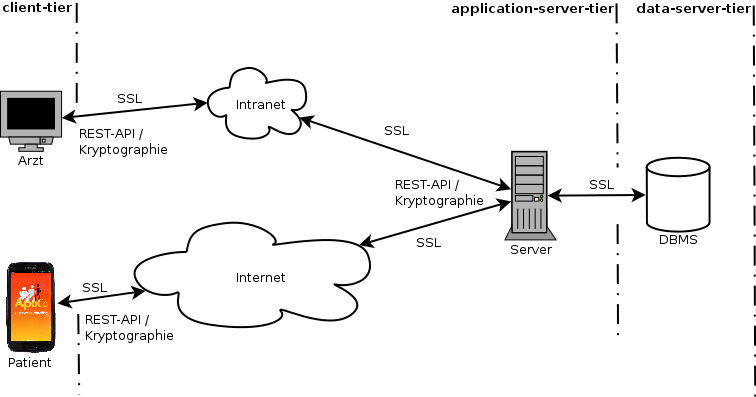
\includegraphics[scale=0.5]{diagramme/kapitel3/gesammt_system.png}
  \caption{Sicherheitskonzept als Diagramm}
 
\end{figure}






